\Week{4}{Proving the Existence : The Probabilistic Method}

The probabilistic method is a simple and powerful technique to show that some combinatorial object with certain properties exists. The idea is quite simple, design a random experiment to obtain the combinatorial object and then show that the probability that the properties does not get satisfied with probability strictly less than 1. Hence, by probability arguments, there must exist the combinatorial object having the properties in the underlying sample space.

\section{Hypergraph 2-coloring}

Now we show the first application of the probablistic method through the example of hypergraph 2-coloring. 
A hypergraph is a pair of two sets $(V,E)$ referred to as vertices and edges (or hyperedges).The edges are subsets of the vertices. If all the sets in $E$ have size $k$, then we call it the $k$-uniform hypergraph. Notice that a graph is a $2$-uniform hypergraph. A proper (vertex) coloring is an assignments of colors to the vertices of a hypergraph so that no edge is monochromatic. Note that this naturally generalizes graph (vertex) coloring where it is insisted that adjacent vertices (that is, the elements of the edges) get different colors.

We show the following theorem using probabilistic method.

\begin{theorem}[\bf Erd\"os~(1963)]
If $H(V,E)$ is a $k$-uniform hypergraph with less than $2^{k-1}$ hyperedges then there exists a proper 2-coloring of $H$.
\end{theorem}
\begin{proof}
Let $H(V,E)$ be a hypergraph such that $|E| < 2^{k-1}$.
The experiment we set up is to color each vertex in the graph with one of the two colors (say red and blue) uniformly at random (that is, with probability $\half$ the vertex will be colored red and with probability $\half$ it will be colored blue). Let $A_e$ be the event that all the $k$ vertices in the hyperedge $e \in E$ gets the same color. We calculate $Pr[A_e]$ first. Since the monochromatic color for $A_e$ can be chosen in two ways: 
$$Pr[A_e] = \frac{2}{2^k} = \frac{1}{2^{k-1}}$$

The coloring is not proper if the event $A_e$ happens for at least one of the hyperedge $e$. Hence, 
$$Pr[\textrm{ coloring is not proper }] \le Pr\left[\bigcup_{e \in E} A_e\right] \le \sum_{e \in E}Pr[A_e] \le \frac{|E|}{2^{k-1}} < 1$$

That is, if we choose a random 2-coloring, we will get a proper-coloring with probability greater than zero. This, in particular implies that there exists a proper $2$-coloring of the hypergraph.
\end{proof}

We remark that by simply restricting $|E| < 2^{k-2}$ we could have proved that if we choose a random 2-coloring, we will get a proper-coloring with probability greater than $\half$. However, this implies that there is even a randomized algorithm to construct the coloring, in this case. Indeed, if we can efficiently derandomize the algorithm, it makes the proof constructive.

The following exercise tells us that the above scheme can also be applied for higher number of colors too.

\begin{exercise}
Suppose $k > 2$ and let $H$ be a $k$-uniform hypergraph with $4^{k-1}$ edges. Show that there is a 4-colouring of $V(H)$ such that no edge is monochromatic.
\end{exercise}

\begin{curiousity}[\textbf{Property-B Conjecture}]
A hypergraph H has \textbf{Property B} (or 2-colorable) if there is a red-blue vertex-coloring with no monochromatic edge. A hypergraph with property B is also called bipartite, by analogy to the bipartite graphs. Erdos (1963) asked: What is the minimum number of edges $m_2(k)$ of a $k$-uniform
hypergraph not having property $B$? Indeed, the above discussion implies that $m_2(k) \ge 2^{k-1}$. Erdos proved an upper bound of $m_2(k) \le O(k^22^k)$. The best known bounds are :
$$\Omega\left(\sqrt{\frac{k}{\ln k}}2^k\right) \le m_2(k) \le O\left(k^22^k\right)$$
The upper bound is due to Erdos (1964) and the lower bound went through a series of improvements to reach the above bound Radhakrishnan and Srinivasan (2000).
$$
\left\{
\begin{array}{c}
m_2(k) \ge \left(\half\right) 2^k \\
\textrm{\cite{Erd63} }
\end{array}
\right\}
\rightarrow
\left\{
\begin{array}{c}
m_2(k) \ge \left(\frac{k}{k+4}\right)2^k \\
\textrm{\cite{Sch64} }
\end{array}
\right\}
\rightarrow
\left\{
\begin{array}{c}
m_2(k) \ge \left(\sqrt[3]{k}\right)2^k \\
\textrm{\cite{Bec78} }
\end{array}
\right\}
\rightarrow
\vspace{-3mm}
\left\{
\begin{array}{l}
m_2(k) \ge \left(\sqrt{\frac{k}{\ln k}}\right)2^k \\[-2mm]
\textrm{[{\color{blue}RS, 2000)}]\nocite{RS00}}
\end{array}
\right\}
$$
It is believed that $k2^k$ is the right asymptotic bound for $m_2(k)$. In fact, this is a conjecture due to Erdos and Lovasz: $m_2(k) \in \Theta(k2^k)$.
\end{curiousity}

\section{Diagonal Ramsey Number Bound}

We now show the original application of the probabilistic method, when it was introduced by Erd\"os. This is to prove a lower bound for certain ramsey numbers. We now quickly introduce Ramsey numbers in this lecture.

The standard starting point is the following brain teaser : any party with at least $6$ people will contain a group of three mutual friends or a group of three mutual non-friends. Indeed, the immediate combinatorial argument goes like this : call the people $1, 2, 3, 4, 5, 6$. Either $1$ has three friends or three non-friends. Without loss of generality, suppose that $2,3,4$ are all friends with $1$. Then if any pair of them are friends with each other, that pair plus $1$ forms a group of three mutual friends. If no two of them are friends, then they are a group of three mutual non-friends. 

Note that the above can also be done graph theoretically where we consider a 6 vertex graph with drawing an edge between two vertices $i,j \in \{1,2,\ldots 6\}$ if and only if they are friends with each other. Now the above argument can be tranlated to graph : \textit{any graph on $6$ vertices will contain either a clique on 3 vertices or an independent set on 3 vertices}.\\[-2mm]

\hspace{-6mm}\begin{minipage}{0.75\textwidth}
An alternate way to represent the above problem is by $2$-coloring the edges of the complete graph $K_6$, by red if the two vertices are friends with each other and with blue otherwise. Now the above statement becomes : {\em in any 2-coloring of $K_n$, there is a monochromatic triangle} - which indeed, is more concise statement.

Is there a peculiarity with $6$ and can the same be argued for $5$? It turns out that we cannot and there is the following counter example (which we represent by the $2$-coloring of $K_5$).
Thus $6$ is the minimum number such that for any $2$-coloring of the edges of $K_6$ there will exist a monochromatic triangle.
\end{minipage}
\begin{minipage}{0.15\textwidth}
\vspace{-3mm}
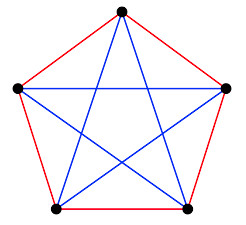
\includegraphics[scale=0.5]{ramsey.jpg}
\end{minipage}

\noindent The Ramsey theory asks a general extremal combinatorics question of this form : For any $s,t \in \mathbb{N}$, what the minimum number $n$ such that there is a guarantee of the form : any $2$-coloring of the edges of the graph $G$ has either a red $K_s$ or a blue $K_t$ in it. This number exists (as proved by Frank Ramsey) and is called the Ramsey Number $R(s,t)$.
In this language, the above argument says $R(3,3) = 6$.
In fact, the existance argument for Ramsey number actually gives the followng upper bound.
\begin{proposition}
$R(s,t) \le R(s,t-1)+R(s-1,t)$.
\end{proposition}

Computing other Ramsey numbers has attracted a lot of attention from combinatorialists. However, we know very little still. $R(s,2)=s$, $43 \le R(5,5) \le 49$ etc. The numbers where $s=t$ are the diagonal entries of the Ramsey matrix (which is natural to imagine given the above). By applyng the above theorem, we have that: $$R(s,s) \le 2^{2s}\sqrt{s}$$

In the rest of this section, we will concetrate on  lower bounds for the diagonal Ramsey numbers. Notice that to show lower bound $R(s,s) \ge n$, we need to show that there is a $2$-coloring of $K_n$ where there is no monochromatic $K_s$. A constructive lower bound of this kind was discovered by Nagy which shows :
$$R(s,s) \ge {s \choose 3}$$

We now apply probabilistic method in order to obtain a stronger lower bound. Erdos, in 1947, introduced
probabilistic methods in his paper {\em Some Remarks on the Theory of Graphs} for proving this lower bound.

\begin{theorem}
The diagonal Ramsey number $R(s,s)$ is at least $\lfloor 2^{\frac{s}{2}}\rfloor$.
Equivalently, when $n=2^{\frac{s}{2}}$, there exists a $2$-coloring of $K_n$ where there is no monochromatic $K_s$.
\end{theorem}
\begin{proof}
As usual, we need to show the existance of a 2-coloring to edges. We set up the following experiment. Color each edge uniformly at random with red or blue. The total number of possible colorings is $2^{n \choose 2}$. The probability of any particular color configuraton is exactly $\frac{1}{2^{n \choose 2}}$.

We need to prove an upper bound of the bad events. Let $S \subseteq n$ of size $s$. Our coloring is bad if $S$ is colored monochromatic under the above coloring.
$$Pr[\textrm{$S$ is monochromatic}] \le \frac{2 \times 2^{{n \choose 2}-{s \choose 2}}}{2^{n \choose 2}} \le 2^{1-{s \choose 2}}$$
$$Pr[\textrm{$\exists S : S$ is monochromatic}] \le
\sum_{S \subseteq [n]:|S|=s} Pr[\textrm{$S$ is monochromatic}] \le {n \choose s}2^{1-{s \choose 2}}$$

If we show that ${n \choose s}2^{1-{s \choose 2}}$ is less than $1$ for $n=2^{s/2}$, then we are done by probablistic argument.

$$
{n \choose s}2^{1-{s \choose 2}} 
\le \frac{n^s}{s!}2^{1-(s/2)+(s^2/s)} 
\le \frac{n^s}{2^{s^2/2}}\frac{2^{1+s/2}}{s!}<1
$$
Hence the proof.
\end{proof}

\begin{exercise-prob}[See Problem Set 2~(Problem~\ref{tournament})]
\begin{show-ps2}{tournament}
A tournament is a directed graph $G(V,E)$ on $n$ vertices where for every pair $(i,j)$, there is either an edge from $i$ to $j$ or from $j$ to $i$, but not both (it represents real tournaments, where we interpret $(i,j)$ directed edge as player $i$ beats player $j$. There is no draw and all pairs of players play a game with each other). 

A tournament T is said to have \textbf{$k$-championship property} if for any set of $k$ vertices in the tournament, there is some vertex in $V$ that has a directed edge to each of those $k$ vertices.

Can $k$-Championship property occur in small tournament graphs? For example, for $k=1$, a tournament will need at least $3$ vertices to have the $k$-Championship property. If $k=2$, a tournament will need at least 5 vertices to have $k$-Championship property.

Show that there are tournments of size $O(k^22^k)$ having $k$-Championship property. [Hint : Consider a random tournament. Fix a set $S$ of $k$ vertices and some vertex $v \notin S$. What is the probability that $v$ is the champion in $S$?]
\end{show-ps2}
\end{exercise-prob}

\begin{exercise-prob}[See Problem Set 2~(Problem~\ref{dominating-set}]
\begin{show-ps2}{dominating-set}
Let $G(V,E)$ be a graph. A set of vertices $D \subseteq V$ is called dominating
with respect to $G$ if every vertex in $V \setminus D$ is adjacent to a vertex in D. $\delta(G)$, the minimum degree amongst $G$’s vertices, is strictly positive. Then $G$ contains a dominating set of size less than or equal to:
$$ \frac{n(1+\log(1+\delta))}{1+\delta} $$
[Hint : Choose a subset $X\subseteq V$ at random (with each vertex in with probability $p$). Let $Y \subseteq V\setminus X$ having no neighbor in $X$. Estimate $X \cup Y$.]
\end{show-ps2}
\end{exercise-prob}